\documentclass[10pt]{article}

\usepackage[paperwidth=30in,paperheight=40in,margin=0.45in]{geometry}
\usepackage[T1]{fontenc}
\usepackage{lmodern}
\usepackage{microtype}
\usepackage{amsmath,amssymb}
\usepackage{graphicx}
\usepackage{tabularx}
\usepackage{multicol}
\usepackage{array}
\usepackage{enumitem}
\usepackage{xcolor}
\usepackage{tikz}
\usetikzlibrary{arrows.meta,positioning,calc,decorations.pathmorphing}
\usepackage{ragged2e}
\usepackage[hidelinks]{hyperref}

\renewcommand{\familydefault}{\sfdefault}

% Muted palette for the review draft.
\definecolor{PosterInk}{HTML}{23313A}
\definecolor{PosterSlate}{HTML}{496577}
\definecolor{PosterSage}{HTML}{657B70}
\definecolor{PosterClay}{HTML}{956B58}
\definecolor{PosterFog}{HTML}{EEF1F2}
\definecolor{PosterSand}{HTML}{F3F0EA}
\definecolor{PosterLine}{HTML}{CCD4D8}
\definecolor{PosterMuted}{HTML}{53616A}

\hypersetup{
  pdftitle={Recovering 3D Vibration Modes from Asynchronous Multi-View Videos},
  colorlinks=true,
  linkcolor=PosterSlate,
  citecolor=PosterSlate,
  urlcolor=PosterSlate
}

\pagestyle{empty}
\setlength{\parindent}{0pt}
\setlength{\parskip}{0.34em}
\setlength{\columnsep}{0.34in}
\setlength{\multicolsep}{0pt}
\setlist[itemize]{leftmargin=1.25em,itemsep=0.15em,topsep=0.15em}
\setlist[enumerate]{leftmargin=1.35em,itemsep=0.18em,topsep=0.18em}

\newcommand{\postersection}[3]{%
  \vspace{0.18in}
  \noindent
  \colorbox{#3}{%
    \parbox{\dimexpr\linewidth-2\fboxsep\relax}{%
      \color{white}\bfseries\fontsize{36}{41}\selectfont
      \strut #1\hspace{0.24em}#2\strut}}
  \vspace{0.11in}
}

\newcommand{\postersubsection}[1]{%
  \vspace{0.10in}
  {\bfseries\color{PosterInk}\fontsize{28}{33}\selectfont #1\par}
  \vspace{0.03in}
}

\newcommand{\smalllabel}[1]{%
  {\bfseries\color{PosterSlate}\fontsize{19}{23}\selectfont\MakeUppercase{#1}}}

\newcommand{\notebox}[3]{%
  \par
  \vspace{0.08in}
  \noindent\fcolorbox{#1}{#2}{%
    \parbox{\dimexpr\linewidth-2\fboxsep-2\fboxrule\relax}{%
      \RaggedRight\vspace{0.05in}\textbf{#3}\vspace{0.05in}}}
  \par
  \vspace{0.08in}
}

\newcommand{\equationbox}[2]{%
  \par
  \vspace{0.06in}
  \noindent\fcolorbox{#1}{PosterFog}{%
    \parbox{\dimexpr\linewidth-2\fboxsep-2\fboxrule\relax}{%
      \vspace{-0.06in}
       \begin{equation*}#2\end{equation*}
       \vspace{-0.09in}}}
  \par
  \vspace{0.06in}
}

\newcommand{\posterplaceholder}[3]{%
  \vspace{0.08in}
  \begin{center}
    \IfFileExists{#1}{%
      \includegraphics[width=\linewidth,height=#2,keepaspectratio]{#1}
    }{%
      \fcolorbox{PosterLine}{PosterFog}{%
        \parbox[c][#2][c]{\dimexpr\linewidth-2\fboxsep-2\fboxrule\relax}{%
          \centering
          {\bfseries\fontsize{22}{27}\selectfont Figure placeholder}\par
          \vspace{0.10in}
          {\fontsize{17}{20}\selectfont\texttt{\detokenize{#1}}}}}}
    \vspace{0.05in}
    {\color{PosterMuted}\fontsize{18}{22}\selectfont #3\par}
  \end{center}
  \vspace{0.06in}
}

\newcommand{\pipelinebox}[4]{%
  \node[draw=#1,fill=#1!7,line width=1.8pt,rounded corners=3pt,
        align=center,text width=2.78in,minimum height=0.66in,#4] (#2)
        {\bfseries\fontsize{17}{20}\selectfont #3};}

\begin{document}
\RaggedRight
\color{PosterInk}
\fontsize{22}{28}\selectfont

% -----------------------------------------------------------------------------
% Header
% -----------------------------------------------------------------------------
\begin{center}
  {\bfseries\fontsize{76}{82}\selectfont
    Recovering 3D Vibration Modes from\\[-0.03in]
    Asynchronous Multi-View Videos\par}
  \vspace{0.15in}
  {\color{PosterSlate}\fontsize{32}{39}\selectfont
    A Gaussian-splat representation connects independently recorded image-space
    vibrations to shared spatial 3D mode shapes.\par}
\end{center}

\vspace{0.16in}
\noindent\colorbox{PosterSand}{%
  \parbox{\dimexpr\linewidth-2\fboxsep\relax}{%
    \centering\fontsize{24}{30}\selectfont
    \textbf{Goal.} Use one mobile phone to scan a static scene and then record
    vibration from several fixed viewpoints at different times. Recover a
    view-consistent, high-detail 3D Gaussian model and a bank of spatial
    vibration fields without requiring synchronized cameras.}}
\vspace{0.12in}

\begin{center}
{\bfseries\color{PosterSlate}\fontsize{22}{26}\selectfont End-to-end pipeline}\par
\vspace{0.04in}
\begin{tikzpicture}[x=1in,y=1in,>=Latex]
  \pipelinebox{PosterSlate}{capture}{1. Sweep + fixed videos}{at={(1.48,0)}}
  \pipelinebox{PosterSlate}{colmap}{2. Joint COLMAP}{at={(5.02,0)}}
  \pipelinebox{PosterSage}{static}{3. Static 3DGS}{at={(8.56,0)}}
  \pipelinebox{PosterClay}{flow}{4. Flow + Fourier modes}{at={(12.10,0)}}
  \pipelinebox{PosterSage}{topology}{5. Pixel--Gaussian topology}{at={(15.64,0)}}
  \pipelinebox{PosterClay}{phase}{6. View phase sync}{at={(19.18,0)}}
  \pipelinebox{PosterSlate}{solve3d}{7. Local 3D solve}{at={(22.72,0)}}
  \pipelinebox{PosterSage}{fill}{8. Motion fill}{at={(26.26,0)}}
  \draw[->,PosterMuted,line width=1.6pt] (capture) -- (colmap);
  \draw[->,PosterMuted,line width=1.6pt] (colmap) -- (static);
  \draw[->,PosterMuted,line width=1.6pt] (static) -- (flow);
  \draw[->,PosterMuted,line width=1.6pt] (flow) -- (topology);
  \draw[->,PosterMuted,line width=1.6pt] (topology) -- (phase);
  \draw[->,PosterMuted,line width=1.6pt] (phase) -- (solve3d);
  \draw[->,PosterMuted,line width=1.6pt] (solve3d) -- (fill);
\end{tikzpicture}
\par
\vspace{0.02in}
{\color{PosterMuted}\fontsize{17}{20}\selectfont
Output: completed complex spatial fields $\phi_k\in\mathbb C^{G\times3}$.\par}
\end{center}
\vspace{0.08in}

% -----------------------------------------------------------------------------
% Two-column poster body
% -----------------------------------------------------------------------------
\begin{multicols}{2}
\RaggedRight

\postersection{1.}{3D Gaussian Splatting}{PosterSlate}

\postersubsection{3D Gaussian Splatting in one paragraph}

3D Gaussian Splatting (3DGS) represents a scene as explicit, oriented,
semi-transparent ellipsoids rather than as a dense voxel grid
(Kerbl et al., 2023). Gaussian $g$ stores
\begin{equation*}
  \mathcal G_g=(\mu_g,\Sigma_g,o_g,c_g),
\end{equation*}
where $\mu_g\in\mathbb R^3$ is its center, $\Sigma_g$ its 3D covariance,
$o_g$ opacity, and $c_g$ appearance. A calibrated camera projects each
Gaussian to an image-space ellipse. Depth-ordered alpha compositing gives
\begin{equation*}
  \widehat C(p)=\sum_{i\in\mathcal H(p)}
  T_{p,i}\,a_{p,i}\,c_i,
  \qquad
  T_{p,i}=\prod_{j<i}(1-a_{p,j}).
\end{equation*}

\begin{center}
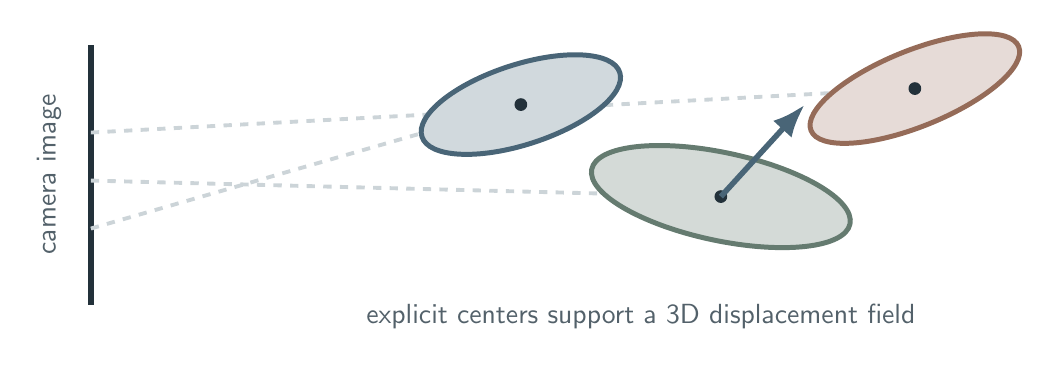
\begin{tikzpicture}[x=1in,y=1in,>=Latex]
  \draw[line width=2pt,PosterInk] (0,0) -- (0,1.30);
  \node[rotate=90,anchor=south,PosterMuted] at (-0.10,0.65)
    {camera image};
  \draw[dashed,PosterLine,line width=1.4pt] (0,0.38) -- (2.15,1.00);
  \draw[dashed,PosterLine,line width=1.4pt] (0,0.62) -- (3.15,0.54);
  \draw[dashed,PosterLine,line width=1.4pt] (0,0.86) -- (4.12,1.08);
  \draw[fill=PosterSlate!25,draw=PosterSlate,line width=1.8pt,
        rotate around={18:(2.15,1.00)}] (2.15,1.00) ellipse (0.52 and 0.20);
  \draw[fill=PosterSage!28,draw=PosterSage,line width=1.8pt,
        rotate around={-12:(3.15,0.54)}] (3.15,0.54) ellipse (0.66 and 0.22);
  \draw[fill=PosterClay!24,draw=PosterClay,line width=1.8pt,
        rotate around={22:(4.12,1.08)}] (4.12,1.08) ellipse (0.56 and 0.19);
  \fill[PosterInk] (2.15,1.00) circle (2.3pt);
  \fill[PosterInk] (3.15,0.54) circle (2.3pt);
  \fill[PosterInk] (4.12,1.08) circle (2.3pt);
  \draw[->,PosterSlate,line width=2pt] (3.15,0.54) -- ++(0.42,0.46);
  \node[align=center,PosterMuted] at (2.75,-0.06)
    {explicit centers support a 3D displacement field};
\end{tikzpicture}
\end{center}

\postersection{2A.}{Modal analysis: coupled motion, simple modes}{PosterSage}

\postersubsection{A two-degree-of-freedom example}

For small displacements around a rest state, a coupled mechanical system is
approximated by
\equationbox{PosterSage}{
  M\ddot u(t)+C\dot u(t)+Ku(t)=f(t).
}
Define the modal transformation
\equationbox{PosterSage}{
  u(t)=\Phi q(t)=\sum_{i=1}^{N}\phi_iq_i(t).
}
Each column $\phi_i$ of $\Phi$ is a spatial \emph{mode shape}; $q_i(t)$ is its
time-varying \emph{modal coordinate}. Substitution and projection by
$\Phi^\top$ give
\equationbox{PosterSage}{
  \begin{gathered}
    \widetilde M\ddot q+\widetilde C\dot q+\widetilde Kq=\widetilde f,\\
    \widetilde X=\Phi^\top X\Phi\ (X=M,C,K),\qquad
    \widetilde f=\Phi^\top f,\\
    \widetilde M,\widetilde K\ \text{diagonal},\qquad
    C\approx\alpha M+\beta K
    \Rightarrow
    \widetilde C\approx\alpha\widetilde M+\beta\widetilde K\ \text{diagonal},\\
    \widetilde m_i\ddot q_i+\widetilde c_i\dot q_i+
    \widetilde k_iq_i=\phi_i^\top f.
  \end{gathered}
}
Modal orthogonality diagonalizes mass and stiffness; Rayleigh damping also
diagonalizes damping. The coupled system therefore separates into independent
modal oscillators.

\begin{center}
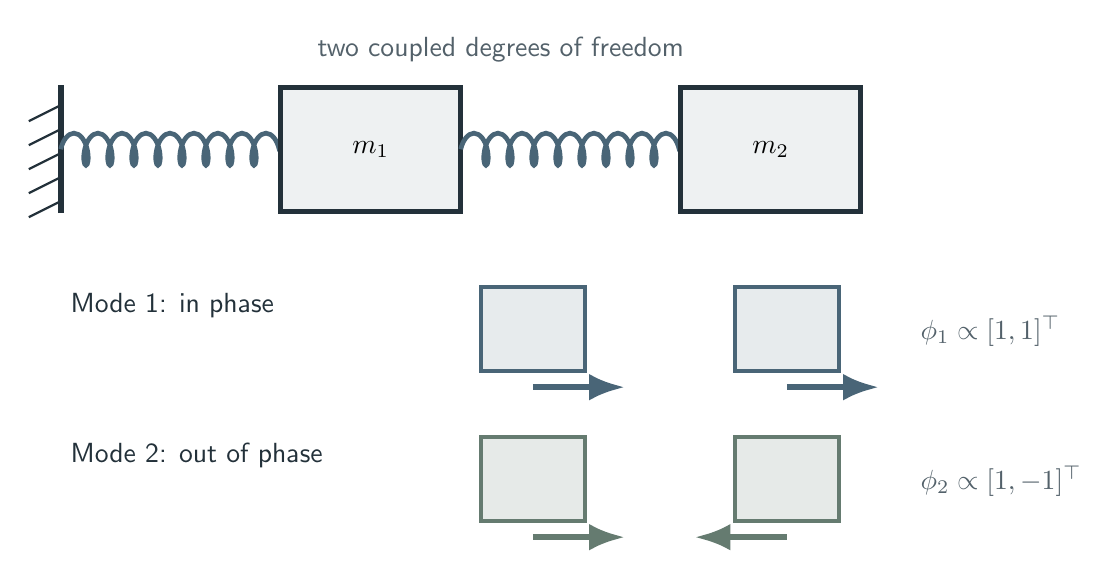
\begin{tikzpicture}[x=1in,y=1in,>=Latex]
  % Physical two-mass system.
  \node[PosterMuted] at (2.30,2.16) {two coupled degrees of freedom};
  \draw[line width=2pt,PosterInk] (0.10,1.34) -- (0.10,1.98);
  \foreach \yy in {1.40,1.52,1.64,1.76,1.88}
    \draw[PosterInk,line width=0.8pt] (0.10,\yy) -- (-0.06,\yy-0.08);
  \draw[decorate,decoration={coil,aspect=0.45,segment length=0.12in,
        amplitude=0.08in},PosterSlate,line width=1.7pt]
        (0.10,1.66) -- (1.20,1.66);
  \draw[fill=PosterFog,draw=PosterInk,line width=1.7pt]
        (1.20,1.35) rectangle (2.10,1.97);
  \node at (1.65,1.66) {$m_1$};
  \draw[decorate,decoration={coil,aspect=0.45,segment length=0.12in,
        amplitude=0.08in},PosterSlate,line width=1.7pt]
        (2.10,1.66) -- (3.20,1.66);
  \draw[fill=PosterFog,draw=PosterInk,line width=1.7pt]
        (3.20,1.35) rectangle (4.10,1.97);
  \node at (3.65,1.66) {$m_2$};

  % Mode 1.
  \node[anchor=west,PosterInk] at (0.10,0.88) {Mode 1: in phase};
  \draw[fill=PosterSlate!13,draw=PosterSlate,line width=1.4pt]
        (2.20,0.55) rectangle (2.72,0.97);
  \draw[fill=PosterSlate!13,draw=PosterSlate,line width=1.4pt]
        (3.47,0.55) rectangle (3.99,0.97);
  \draw[->,PosterSlate,line width=2.2pt] (2.46,0.47) -- ++(0.46,0);
  \draw[->,PosterSlate,line width=2.2pt] (3.73,0.47) -- ++(0.46,0);
  \node[anchor=west,PosterMuted] at (4.35,0.75) {$\phi_1\propto[1,1]^\top$};

  % Mode 2.
  \node[anchor=west,PosterInk] at (0.10,0.13) {Mode 2: out of phase};
  \draw[fill=PosterSage!16,draw=PosterSage,line width=1.4pt]
        (2.20,-0.20) rectangle (2.72,0.22);
  \draw[fill=PosterSage!16,draw=PosterSage,line width=1.4pt]
        (3.47,-0.20) rectangle (3.99,0.22);
  \draw[->,PosterSage,line width=2.2pt] (2.46,-0.28) -- ++(0.46,0);
  \draw[->,PosterSage,line width=2.2pt] (3.73,-0.28) -- ++(-0.46,0);
  \node[anchor=west,PosterMuted] at (4.35,0.00) {$\phi_2\propto[1,-1]^\top$};
\end{tikzpicture}
\end{center}

\postersection{2B.}{Modal analysis from ordinary video}{PosterSage}

\postersubsection{Davis et al.: image-space modal bases}

Davis, Chen, and Durand recover projections of resonant modes from a short
video without knowing geometry or material parameters (Davis et al., 2015).
Their key observation is that, near a resonant
frequency $\omega_i$, the temporal spectrum of visible displacement is
proportional to the projected mode shape:
\equationbox{PosterSage}{
  VU(\omega_i)=A_iH_i(\omega_i)V\phi_i
  \quad\Longrightarrow\quad
  VU(\omega_i)\propto V\phi_i.
}
Here $V$ selects visible degrees of freedom, $A_i$ is the unknown excitation at
the mode, and $H_i$ is its frequency response. The pipeline is:

\begin{center}
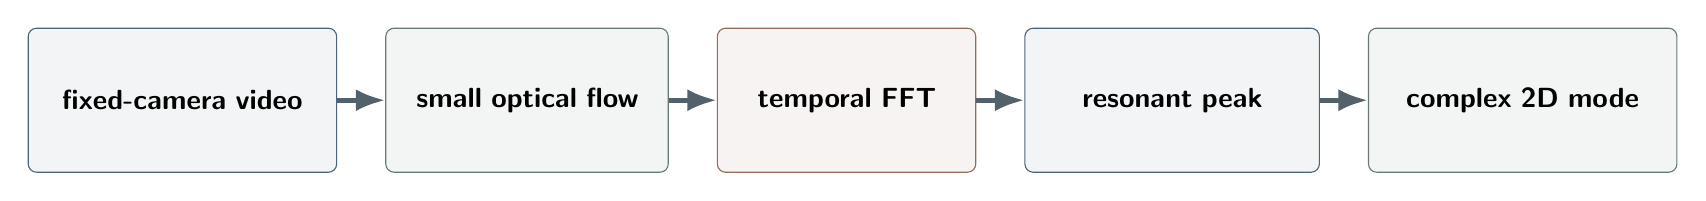
\begin{tikzpicture}[node distance=0.24in,>=Latex]
  \node[draw=PosterSlate,fill=PosterSlate!7,rounded corners=3pt,
        text width=1.45in,minimum height=0.72in,align=center] (video)
        {\bfseries fixed-camera video};
  \node[draw=PosterSage,fill=PosterSage!8,rounded corners=3pt,
        text width=1.32in,minimum height=0.72in,align=center,right=of video] (flow)
        {\bfseries small optical flow};
  \node[draw=PosterClay,fill=PosterClay!8,rounded corners=3pt,
        text width=1.20in,minimum height=0.72in,align=center,right=of flow] (fft)
        {\bfseries temporal FFT};
  \node[draw=PosterSlate,fill=PosterSlate!7,rounded corners=3pt,
        text width=1.38in,minimum height=0.72in,align=center,right=of fft] (peak)
        {\bfseries resonant peak};
  \node[draw=PosterSage,fill=PosterSage!8,rounded corners=3pt,
        text width=1.45in,minimum height=0.72in,align=center,right=of peak] (mode)
        {\bfseries complex 2D mode};
  \draw[->,line width=1.7pt,PosterMuted] (video) -- (flow);
  \draw[->,line width=1.7pt,PosterMuted] (flow) -- (fft);
  \draw[->,line width=1.7pt,PosterMuted] (fft) -- (peak);
  \draw[->,line width=1.7pt,PosterMuted] (peak) -- (mode);
\end{tikzpicture}
\end{center}

Each spatial slice of the displacement FFT is a candidate mode. Peaks in the
global power spectrum identify resonances; magnitude visualizes motion strength
and complex phase records relative timing. These projected modes need not be
orthogonal or purely real; Davis retains complex, non-binary phase relationships
when they better explain the video. The selected modes become a basis for
synthesizing 2D image deformation:
\begin{equation*}
  D(t)=\sum_i\operatorname{Re}\{\phi_i' q_i(t)\}.
\end{equation*}

\posterplaceholder{../poster_brief/figures/bush_flow_and_frequency.png}{2.72in}{%
  Bush fixed-view optical flow, power spectrum, and one selected complex 2D mode.}

\postersubsection{What makes the Davis derivation possible?}

{\renewcommand{\arraystretch}{1.16}
\fontsize{21}{26}\selectfont
\begin{tabularx}{\linewidth}{@{}>{\bfseries\color{PosterSlate}}p{0.28\linewidth}>{\RaggedRight\arraybackslash}X@{}}
Small linear motion
  & The object vibrates near a fixed rest state, so superposition applies. \\
Weak perspective
  & Small 3D displacement projects approximately linearly into the image. \\
Well-spaced modes
  & Resonances do not strongly overlap, so one frequency isolates one mode. \\
Broad-spectrum forcing
  & The observed excitation is sufficiently rich; unknown force/mass scaling is
    absorbed into a global modal scale. \\
\end{tabularx}}

\postersection{3.}{Why asynchronous multi-view is different}{PosterClay}

Synchronized camera arrays can triangulate the same moving surface at the same
instant and recover detailed dynamic 3D scenes. Most users, however, own one
phone. They can revisit several viewpoints, but the recordings start at
different times and experience different forcing.

\begin{center}
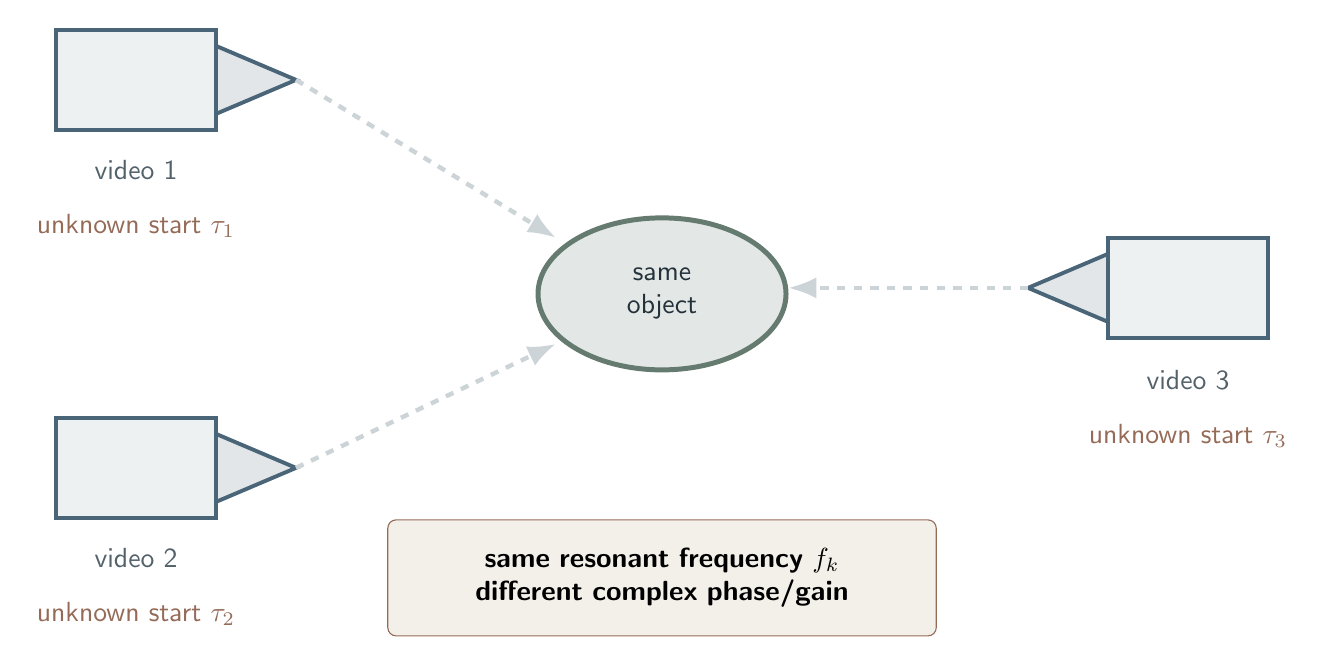
\begin{tikzpicture}[x=1in,y=1in,>=Latex]
  % Central object.
  \draw[fill=PosterSage!18,draw=PosterSage,line width=1.8pt]
        (3.25,1.30) ellipse (0.62 and 0.38);
  \node[PosterInk,align=center] at (3.25,1.30) {same\\object};
  % Camera 1.
  \draw[fill=PosterFog,draw=PosterSlate,line width=1.6pt]
        (0.22,2.12) rectangle (1.02,2.62);
  \draw[fill=PosterSlate!16,draw=PosterSlate,line width=1.4pt]
        (1.02,2.20) -- (1.42,2.37) -- (1.02,2.54) -- cycle;
  \node[PosterMuted] at (0.62,1.92) {video 1};
  \node[PosterClay] at (0.62,1.64) {unknown start $\tau_1$};
  \draw[->,dashed,PosterLine,line width=1.6pt] (1.42,2.37) -- (2.72,1.58);
  % Camera 2.
  \draw[fill=PosterFog,draw=PosterSlate,line width=1.6pt]
        (0.22,0.18) rectangle (1.02,0.68);
  \draw[fill=PosterSlate!16,draw=PosterSlate,line width=1.4pt]
        (1.02,0.26) -- (1.42,0.43) -- (1.02,0.60) -- cycle;
  \node[PosterMuted] at (0.62,-0.02) {video 2};
  \node[PosterClay] at (0.62,-0.30) {unknown start $\tau_2$};
  \draw[->,dashed,PosterLine,line width=1.6pt] (1.42,0.43) -- (2.72,1.05);
  % Camera 3.
  \draw[fill=PosterFog,draw=PosterSlate,line width=1.6pt]
        (5.48,1.08) rectangle (6.28,1.58);
  \draw[fill=PosterSlate!16,draw=PosterSlate,line width=1.4pt]
        (5.48,1.16) -- (5.08,1.33) -- (5.48,1.50) -- cycle;
  \node[PosterMuted] at (5.88,0.87) {video 3};
  \node[PosterClay] at (5.88,0.59) {unknown start $\tau_3$};
  \draw[->,dashed,PosterLine,line width=1.6pt] (5.08,1.33) -- (3.88,1.33);
  % Shared frequency label.
  \node[draw=PosterClay,fill=PosterSand,rounded corners=3pt,
        text width=2.65in,minimum height=0.58in,align=center]
        at (3.25,-0.12)
        {\bfseries same resonant frequency $f_k$\\different complex phase/gain};
\end{tikzpicture}
\end{center}

Time-domain optical flow from these recordings is not synchronized and should
not match frame by frame. Our central modeling assumption is weaker:

\notebox{PosterClay}{PosterSand}{%
  \textbf{Frequency-domain consistency assumption.} If geometry, boundary
  conditions, and material properties do not change between recordings, the
  same natural frequency represents the same underlying 3D spatial mode.
  Each view may observe it with a different complex phase and amplitude.}

\postersubsection{Additional assumptions introduced by our setting}

\begin{itemize}
  \item A static sweep defines one canonical rest geometry.
  \item Fixed reference cameras can be calibrated into that coordinate system.
  \item Vibrations remain small enough for camera and modal linearization.
  \item The same modes are excited across takes, although forcing strength and
        phase may differ.
  \item Frequencies are stable and sufficiently separated over the capture.
\end{itemize}

\postersection{4.}{Solving shared 3D modes}{PosterSlate}

\postersubsection{A. Shared canonical scene}

We sample a sweep video and add one reference image from each fixed view to the
same COLMAP reconstruction. This provides a common world coordinate system.
Registered sweep views train a foreground/background 3DGS; fixed cameras are
exported for modal projection.

\posterplaceholder{../poster_brief/figures/bush_capture_and_cameras.png}{1.55in}{%
  Sweep frames, fixed references, and registered cameras around the canonical scene.}

\postersubsection{B. Frequency evidence and observation topology}

Foreground optical flow is transformed over time:
\begin{equation*}
  \widehat d_{v,p}(f)=\sum_t d_{v,p}(t)e^{-i2\pi ft}.
\end{equation*}
Greedy frequency selection chooses a compact set that reconstructs the observed
flow spectra. Rendered foreground depth unprojects each retained pixel to a
canonical surface point $X_{v,p}$. Nearby Gaussians are ranked by
\begin{equation*}
  s_{v,p,g}=o_g\exp\!\left[-\tfrac12
  (X_{v,p}-\mu_g)^\top\Sigma_g^{-1}(X_{v,p}-\mu_g)\right].
\end{equation*}
This creates a mode-independent observation topology connecting complex 2D
measurements to plausible foreground Gaussian centers.

\postersubsection{C. Synchronizing phase without synchronized time}

At frequency $k$, view $v$ observes a complex 2D displacement
$\widehat d_{v,k,p}$. For a Gaussian point $g$ with complex 3D mode vector
$\phi_{k,g}$, first-order camera projection gives
\equationbox{PosterClay}{
  \widehat d_{v,k,p}\approx
  \alpha_{v,k}J_{v,g}\phi_{k,g},
}
where $J_{v,g}\in\mathbb R^{2\times3}$ is the camera projection Jacobian and
$\alpha_{v,k}\in\mathbb C$ is the unknown view-specific phase/gain.

Directly optimizing both $\phi$ and every $\alpha$ is bilinear. We instead set
$\beta_{v,k}=\alpha_{v,k}^{-1}$ and use points observed by multiple cameras.
For one shared Gaussian, weighted equations can be stacked as
\equationbox{PosterClay}{
  A_g\phi_{k,g}=B_g\beta_k.
}
The columns of $B_g$ place each view's measured complex flow in the
corresponding view block. Let $N_g$ span the left null space of the stacked
Jacobian $A_g$:
\begin{equation*}
  N_g^HA_g=0.
\end{equation*}
Any set of view offsets that can be explained by one common 3D displacement
must therefore satisfy
\equationbox{PosterClay}{
  N_g^HB_g\beta_k=0.
}

\begin{center}
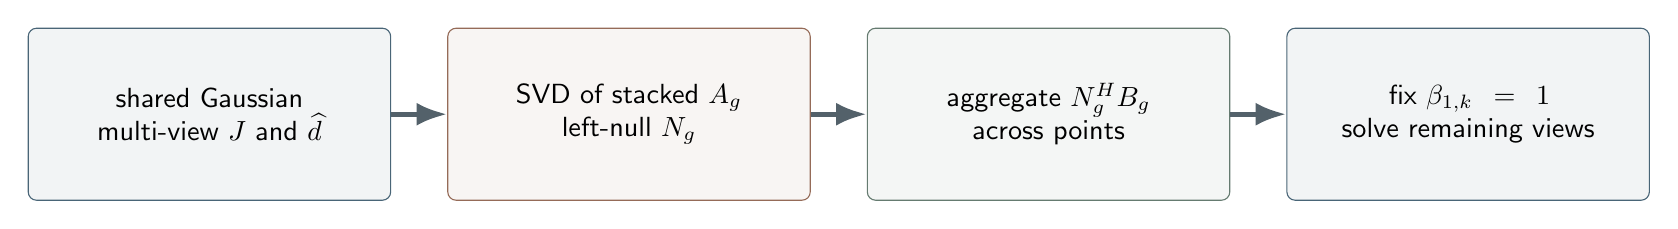
\begin{tikzpicture}[node distance=0.28in,>=Latex]
  \node[draw=PosterSlate,fill=PosterSlate!7,rounded corners=3pt,
        text width=1.72in,minimum height=0.86in,align=center] (shared)
        {shared Gaussian\\multi-view $J$ and $\widehat d$};
  \node[draw=PosterClay,fill=PosterClay!7,rounded corners=3pt,
        text width=1.72in,minimum height=0.86in,align=center,right=of shared] (null)
        {SVD of stacked $A_g$\\left-null $N_g$};
  \node[draw=PosterSage,fill=PosterSage!7,rounded corners=3pt,
        text width=1.72in,minimum height=0.86in,align=center,right=of null] (aggregate)
        {aggregate $N_g^HB_g$\\across points};
  \node[draw=PosterSlate,fill=PosterSlate!7,rounded corners=3pt,
        text width=1.72in,minimum height=0.86in,align=center,right=of aggregate] (solve)
        {fix $\beta_{1,k}=1$\\solve remaining views};
  \draw[->,PosterMuted,line width=1.8pt] (shared) -- (null);
  \draw[->,PosterMuted,line width=1.8pt] (null) -- (aggregate);
  \draw[->,PosterMuted,line width=1.8pt] (aggregate) -- (solve);
\end{tikzpicture}
\end{center}

We aggregate these constraints over many shared points, fix one reference-view
gauge $\beta_{1,k}=1$, and solve a robust least-squares synchronization. The
default model estimates unit-magnitude phase offsets; a bounded-complex option
also allows limited gain differences. Rank and information tests exclude views
whose phase is not identifiable from the available shared geometry.

\notebox{PosterClay}{PosterFog}{%
  \textbf{Interpretation.} The left-null projection removes the unknown 3D
  vector from the synchronization step. It asks only whether the differently
  phased 2D observations could have come from \emph{some} common 3D motion.}

\postersubsection{D. Spatial structure, local solve, and completion}

Mutual KNN edges are removed across strong Gaussian-color or rendered-depth
discontinuities. Remaining connected neighborhoods provide local structure.
For a local first-order rigid component $c$,
\begin{equation*}
  \phi_{k,g}=B_{c,g}\xi_{k,c},
\end{equation*}
and the complex twist is obtained by matching its projections to all aligned
2D observations:
{\fontsize{20}{24}\selectfont
\begin{equation*}
  \xi_{k,c}^{\star}=\arg\min_{\xi}
  \sum_{(v,p,g)\in\mathcal O_c}\bar w_{v,p,g}
  \left\|\alpha_{v,k}J_{v,g}B_{c,g}\xi-
  \widehat d_{v,k,p}\right\|_2^2.
\end{equation*}}
A separate foreground graph propagates trusted observed motion into compatible
unobserved Gaussians while preserving the measured solution.

\posterplaceholder{../poster_brief/figures/bush_rigid_components.png}{1.75in}{%
  Bush Gaussian graph colored by local component or observation support.}

\posterplaceholder{../poster_brief/figures/bush_modes_grid.png}{2.75in}{%
  Representative completed Bush spatial 3D modes, shown from a common view and scale.}

\notebox{PosterSlate}{PosterSand}{%
  \textbf{Current interpretation.} The output modes are evidence-driven,
  spatially coherent complex displacement patterns. They are not yet mass- and
  stiffness-normalized structural eigenmodes. Accuracy depends on camera
  calibration, masks, optical flow, static Gaussian quality, and the validity
  of the shared-frequency assumption.}

\end{multicols}

\end{document}
